%%%%%%%%%%%%%%%%%%%%%%%%%%%%%%%%%%%%%%%%%
% Beamer Presentation
% LaTeX Template
% Version 1.0 (10/11/12)
%
% This template has been downloaded from:
% http://www.LaTeXTemplates.com
%
% License:
% CC BY-NC-SA 3.0 (http://creativecommons.org/licenses/by-nc-sa/3.0/)
%
%%%%%%%%%%%%%%%%%%%%%%%%%%%%%%%%%%%%%%%%%

%----------------------------------------------------------------------------------------
%	PACKAGES AND THEMES
%----------------------------------------------------------------------------------------

\documentclass{beamer}

\mode<presentation> {

% The Beamer class comes with a number of default slide themes
% which change the colors and layouts of slides. Below this is a list
% of all the themes, uncomment each in turn to see what they look like.

%\usetheme{default}
%\usetheme{AnnArbor}
%\usetheme{Antibes}
%\usetheme{Bergen}
%\usetheme{Berkeley}
%\usetheme{Berlin}
%\usetheme{Boadilla}
%\usetheme{CambridgeUS}
%\usetheme{Copenhagen}
%\usetheme{Darmstadt}
%\usetheme{Dresden}
%\usetheme{Frankfurt}
%\usetheme{Goettingen}
%\usetheme{Hannover}
%\usetheme{Ilmenau}
%\usetheme{JuanLesPins}
%\usetheme{Luebeck}
\usetheme{Madrid}
%\usetheme{Malmoe}
%\usetheme{Marburg}
%\usetheme{Montpellier}
%\usetheme{PaloAlto}
%\usetheme{Pittsburgh}
%\usetheme{Rochester}
%\usetheme{Singapore}
%\usetheme{Szeged}
%\usetheme{Warsaw}

% As well as themes, the Beamer class has a number of color themes
% for any slide theme. Uncomment each of these in turn to see how it
% changes the colors of your current slide theme.

%\usecolortheme{albatross}
%\usecolortheme{beaver}
%\usecolortheme{beetle}
%\usecolortheme{crane}
%\usecolortheme{dolphin}
%\usecolortheme{dove}
%\usecolortheme{fly}
%\usecolortheme{lily}
%\usecolortheme{orchid}
%\usecolortheme{rose}
%\usecolortheme{seagull}
%\usecolortheme{seahorse}
%\usecolortheme{whale}
%\usecolortheme{wolverine}

%\setbeamertemplate{footline} % To remove the footer line in all slides uncomment this line
%\setbeamertemplate{footline}[page number] % To replace the footer line in all slides with a simple slide count uncomment this line

%\setbeamertemplate{navigation symbols}{} % To remove the navigation symbols from the bottom of all slides uncomment this line
}

\usepackage{graphicx} % Allows including images
\usepackage{booktabs} % Allows the use of \toprule, \midrule and \bottomrule in tables
\usepackage{geometry}%????
\usepackage{graphics}%????
\usepackage{caption}%????
\usepackage{caption}
\usepackage{colortbl}
\usepackage{color}
\usepackage{array}
\usepackage{graphicx} 
\usepackage{subfigure} 

%----------------------------------------------------------------------------------------
%	TITLE PAGE
%----------------------------------------------------------------------------------------

\title[Bodyfat prediction]{Bodyfat prediction} % The short title appears at the bottom of every slide, the full title is only on the title page

\author{Y. Tang, H. Xia, Y. Zheng} % Your name
\institute[UWM] % Your institution as it will appear on the bottom of every slide, may be shorthand to save space
{
University of Wisconsin-Madison \\ % Your institution for the title page
}
\date{\today} % Date, can be changed to a custom date

\begin{document}

\begin{frame}
\titlepage % Print the title page as the first slide
\end{frame}

\begin{frame}
\frametitle{Introduction}
\begin{itemize}
\item dataset: Y=body fat Percentage;
               X=14 physical measurements 
\item model: a two-term nonlinear model
\end{itemize}

\end{frame}


%------------------------------------------------

\begin{frame}
\frametitle{Data Cleaning}
\begin{itemize}
\item Summary of variables

\begin{figure}[h]
   \centering
   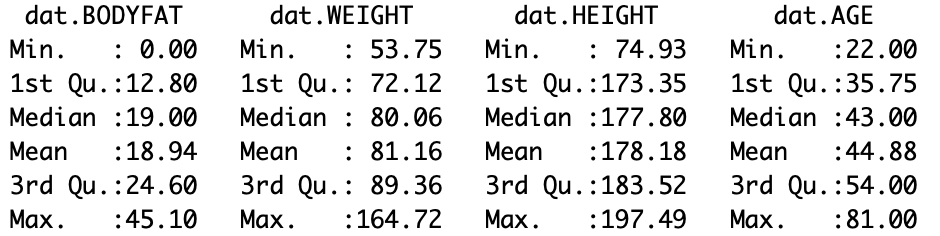
\includegraphics[scale=0.5]{picture1.png}
   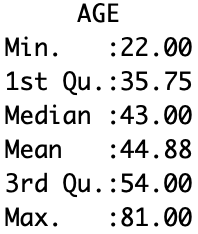
\includegraphics[scale=0.5]{picture2.png}
   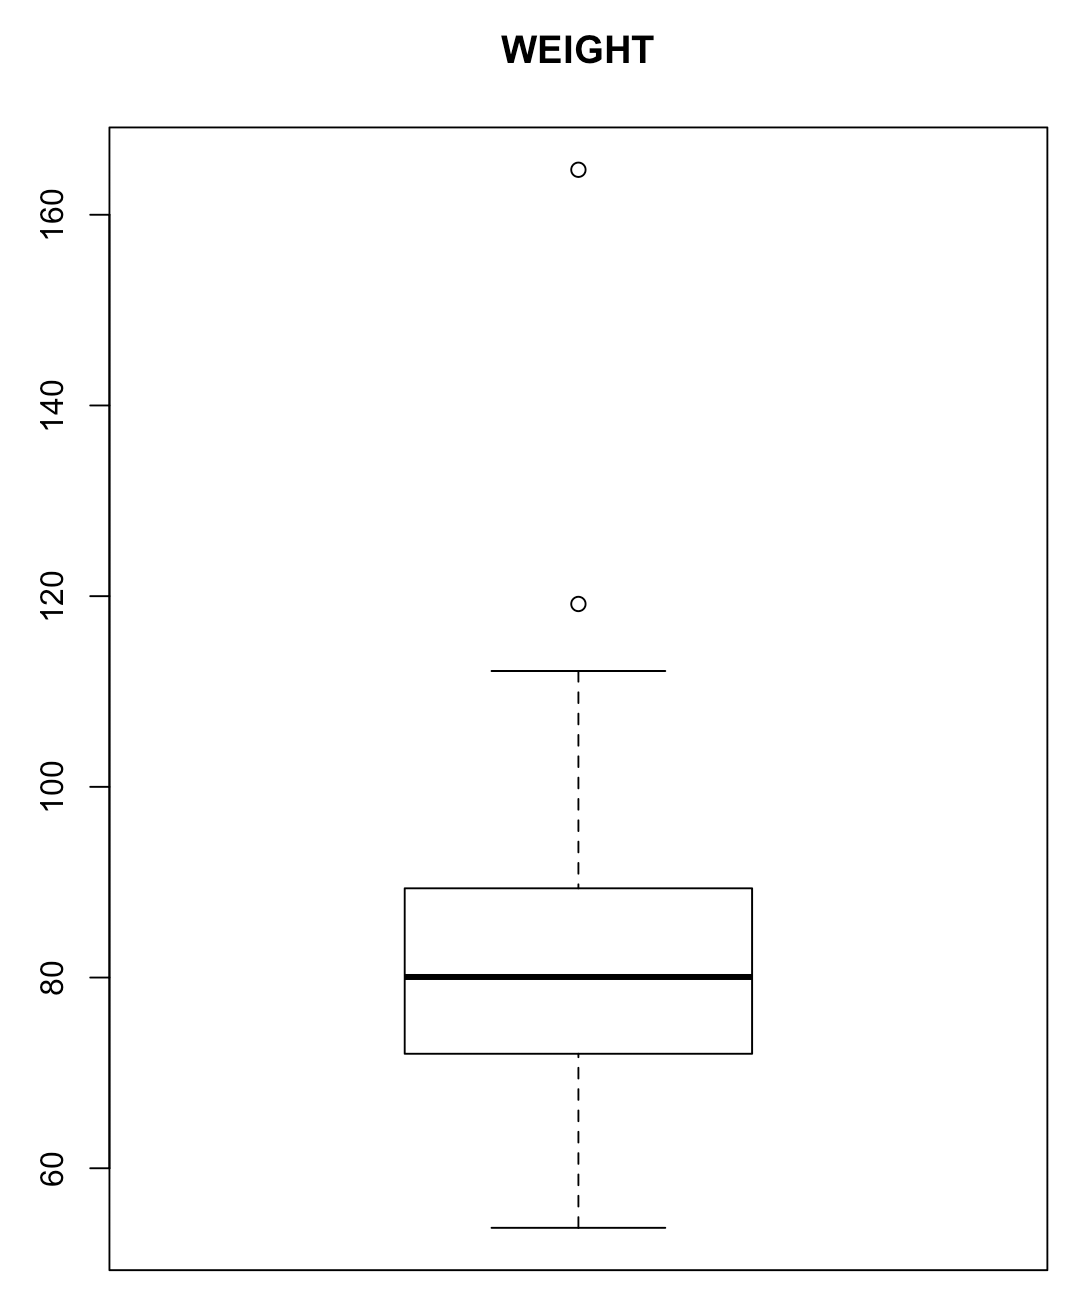
\includegraphics[scale=0.15]{picture5.png}
\end{figure}
\begin{figure}[h]
   \centering
   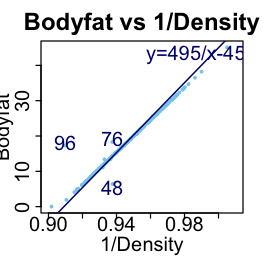
\includegraphics[scale=0.5]{picture3.png}
   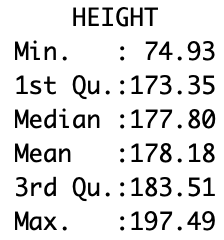
\includegraphics[scale=0.5]{icture4.png}
   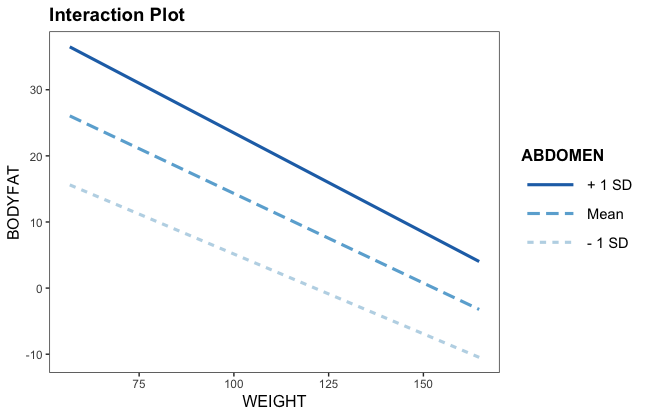
\includegraphics[scale=0.15]{picture6.png}
\end{figure}
\end{itemize}
\end{frame}


%------------------------------------------------
\begin{frame}{Data Cleaning}
\begin{itemize}
\item four weird records 

\begin{table}
\begin{tabular}{l p{6cm} p{6cm}}
\hline
39 & weight=164.72 lbs \\
42 & height=74.93 inch \\
79 & age=81 years old \\
182 & bodyfat=0


\end{tabular}
\end{table}
\end{itemize}
\end{frame}


%------------------------------------------------
\begin{frame}{Data Cleaning}
\begin{itemize}
    \item Consistency of BMI versus HEIGHT and WEIGHT
        \[ BMI=\frac{WEIGHT}{(\frac{HEIGHT}{100})^2} \]
\end{itemize}    
We change the height of 42th but retain 39th and 79th because it seems that the 79th is a normal thin old man, the 39th is a very heavy man which follows the bmi equation. 
\end{frame}
%------------------------------------------------
\begin{frame}{Data Cleaning}
\begin{itemize}
    \item Consistency between DENSITY and BODYFAT
    \begin{figure}[h]
    \centering
    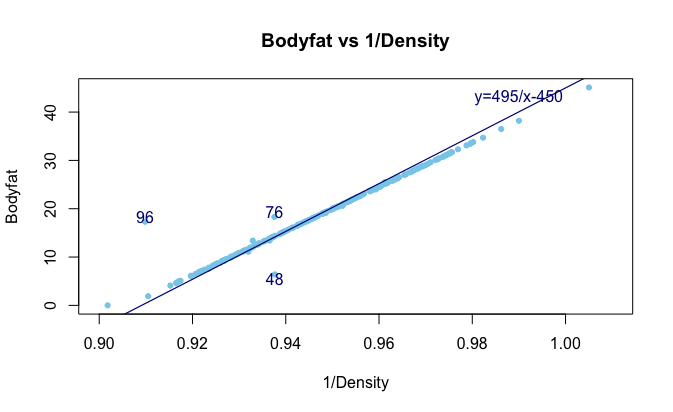
\includegraphics[scale=0.5]{picture7.png}
    \end{figure}
\end{itemize}
    
\end{frame}

%------------------------------------------------

\begin{frame}
\frametitle{Variable Selection}
Forward stepwise variables selection based on AIC\\

\begin{table}
\begin{center}
\begin{tabular}{lll}
\toprule
Num. of Variables & Variables Selected & AIC \\
\midrule
1 & Abdomen & 757.29\\
2 & Abdomen, Weight & 712.53\\
3 & Abdomen, Weight, Wrist & 706.45\\
4 & Abdomen, Weight, Wrist, Forearm & 702.18\\
\bottomrule
\end{tabular}
\end{center}
\end{table}

\end{frame}

%------------------------------------------------
\begin{frame}
\frametitle{Bodyfat, Abdomen, Weight, Wrist Relationships}

\begin{figure}[h]
   \centering
   \includegraphics[width=12cm,height=8cm]{Picture1.pdf}
\end{figure}

\end{frame}

%------------------------------------------------
\begin{frame}
\frametitle{Interaction Effect}

\begin{figure}[h]
   \centering
   \includegraphics[width=5.6cm,height=6cm]{Picture2.pdf}
   \includegraphics[width=5.6cm,height=6cm]{Picture3.pdf}
\end{figure}

\end{frame}

%------------------------------------------------

\begin{frame}
\frametitle{Model Comparison}

\begin{table}
\begin{center}
\begin{tabular}{lll}
\toprule
Model & Adj.R-squared & MSE \\
\midrule
m2\_ridge & 0.7127 & 16.69\\
m3 & 0.7185 & 16.16\\
m5 & 0.7258 & 15.80\\
\bottomrule
\end{tabular}
\end{center}
\end{table}

\end{frame}



%------------------------------------------------


\begin{frame}
\frametitle{Model Comparison}
\begin{itemize}
\item Final Model
\end{itemize}

$$ Bodyfat(\%) = -45.3249 + 0.9092\times Abdomen(cm)

\qquad \qquad \qquad \qquad \qquad \qquad -0.0133\times Weight(kg)\times Wrist(cm)$$ 

\begin{table}
\begin{center}
\begin{tabular}{cccccc}
\toprule
&     Estimate & Std.Error & t.value & P.value \\
\midrule
Intercept &  -45.3249 & 2.573 & -17.62 & \<2e-16 \\
$ABDOMEN$  & 0.9092 & 0.047 & 19.42 & \<2e-16 \\
$WEIGHT:WRIST$ &  -0.0133 & 0.002 & -8.22 & 1.14e-14 \\


\bottomrule
\end{tabular}
\end{center}
\end{table}

\end{frame}

%------------------------------------------------

\begin{frame}
\frametitle{Model Diagnostic}
\begin{itemize}
\item Normality Assumption

$H_{0}$: the residual follows normal distribution.


\item Homoscedasticity Assumption

$H_{0}$: homoscedasticity vs $H_{1}$:variance residuals vary with the level of fitted values

\begin{table}
\small
\begin{center}
\begin{tabular}{cccccc}
\toprule
Shapiro-Wilk normality test & Non-constant Variance Score Test  \\
\midrule
W = 0.99056 & Chisquare = 0.0001924752, Df = 1  \\
p-value = 0.1039 & p = 0.98893  \\

\bottomrule
\end{tabular}
\end{center}
\end{table}

\begin{figure}[h]
   \centering
   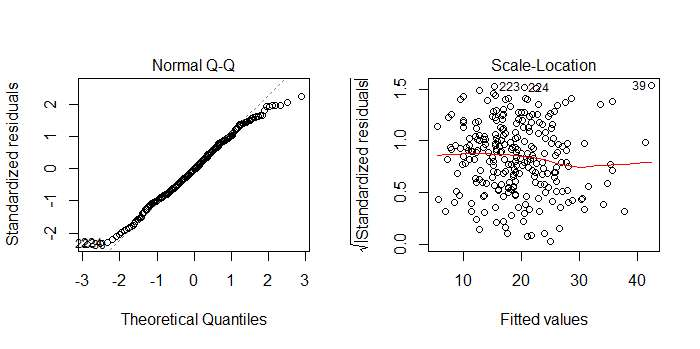
\includegraphics[width=8cm,height=3.6cm]{Picture4.png}
\end{figure}

\end{itemize}
\end{frame}

%------------------------------------------------

\begin{frame}
\frametitle{Model Diagnostic}
\begin{itemize}
\item Robustness

rlm(formula = $BODYFAT$ \~{} $ABDOMEN$ + $WEIGHT:WRIST$)

\begin{table}
\begin{center}
\begin{tabular}{cccccc}
\toprule
   &   coefficients from m5 & coefficients from rlm5 \\
\midrule
Intercept &  -45.325 &  -46.652  \\
$ABDOMEN$  & 0.909 & 0.922  \\
$WEIGHT:WRIST$ &  -0.013 & -0.013 &  \\

\bottomrule
\end{tabular}
\end{center}
\end{table}

The coefficients of the robust model5 are very close to those of the previous model5, which means model5 is robust to some extent.

\end{itemize}
\end{frame}

%------------------------------------------------

\begin{frame}
\frametitle{Rules of thumb}
$$ Bodyfat(\%) = -45.3249 + 0.9092\times Abdomen(cm)

\qquad \qquad \qquad \qquad \qquad \qquad -0.0133\times Weight(kg)\times Wrist(cm)$$ \\
$$ Bodyfat(\%) = -45 + 0.91\times Abdomen(cm) -0.013\times Weight(kg)\times Wrist(cm)$$

\begin{itemize}
\item Explain the practical meaning of this model:

For a 75 kg man whose abdomen is 85 cm, wrist is 18 cm, his predicted bodyfat is around 14.97\%. There is a 95\% probability that his bodyfat is between 14.35\% and 15.59\%. Second model is a simpler one to calculate bodyfat, it predicts this person has 14.8\% bodyfat.

\end{itemize}
\end{frame}

%------------------------------------------------
\begin{frame}
\frametitle{\ }
$$Thank\quad you!$$
\end{frame}
%------------------------------------------------
\end{document}